\begin{frame}
  \frametitle{Základní předpoklady}
  
  \begin{itemize}
  	\item Neutrony lze popsat jako bodové objekty, ovlivněné pouze jadernými silami
  	\begin{itemize}
  		\item[\Rabullet] pohyb neutronů po přímých drahách
  		\item[\Rabullet] interakce s okolními atomy vede k záchytu či změně směru anebo rychlosti neutronu
  	\end{itemize}
  	\item Vzájemné interakce mezi neutrony jsou zanedbatelné
  	\item Izotropní prostředí, atomy sféricky symetrické
  	\begin{itemize}
  		\item samotný rozptyl a pohyb neutronů však může být anizotropní
  	\end{itemize}
  	\item Stacionární rozložení atomů (zanedbáváme tepelný pohyb)
  \end{itemize}

  \uncover<2->{
    \alert{Pohyb neutronů prostředím lze popsat lineární Boltzmannovou rovnicí}
    \begin{center}
    	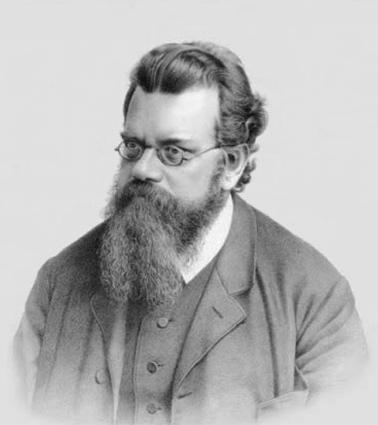
\includegraphics[scale=0.30]{obr/Boltzmann.jpg}
    \end{center}
  }
  
\end{frame}

\begin{frame}[t]
  \frametitle{Stavový prostor}
 
  $$
    X = \VV \times \EE \times \SS \equiv \{x = (\br,E,\bomega):\ \br\in \VV, E \in \EE, \bomega\in \SS\}
  $$
  
  \begin{center}
	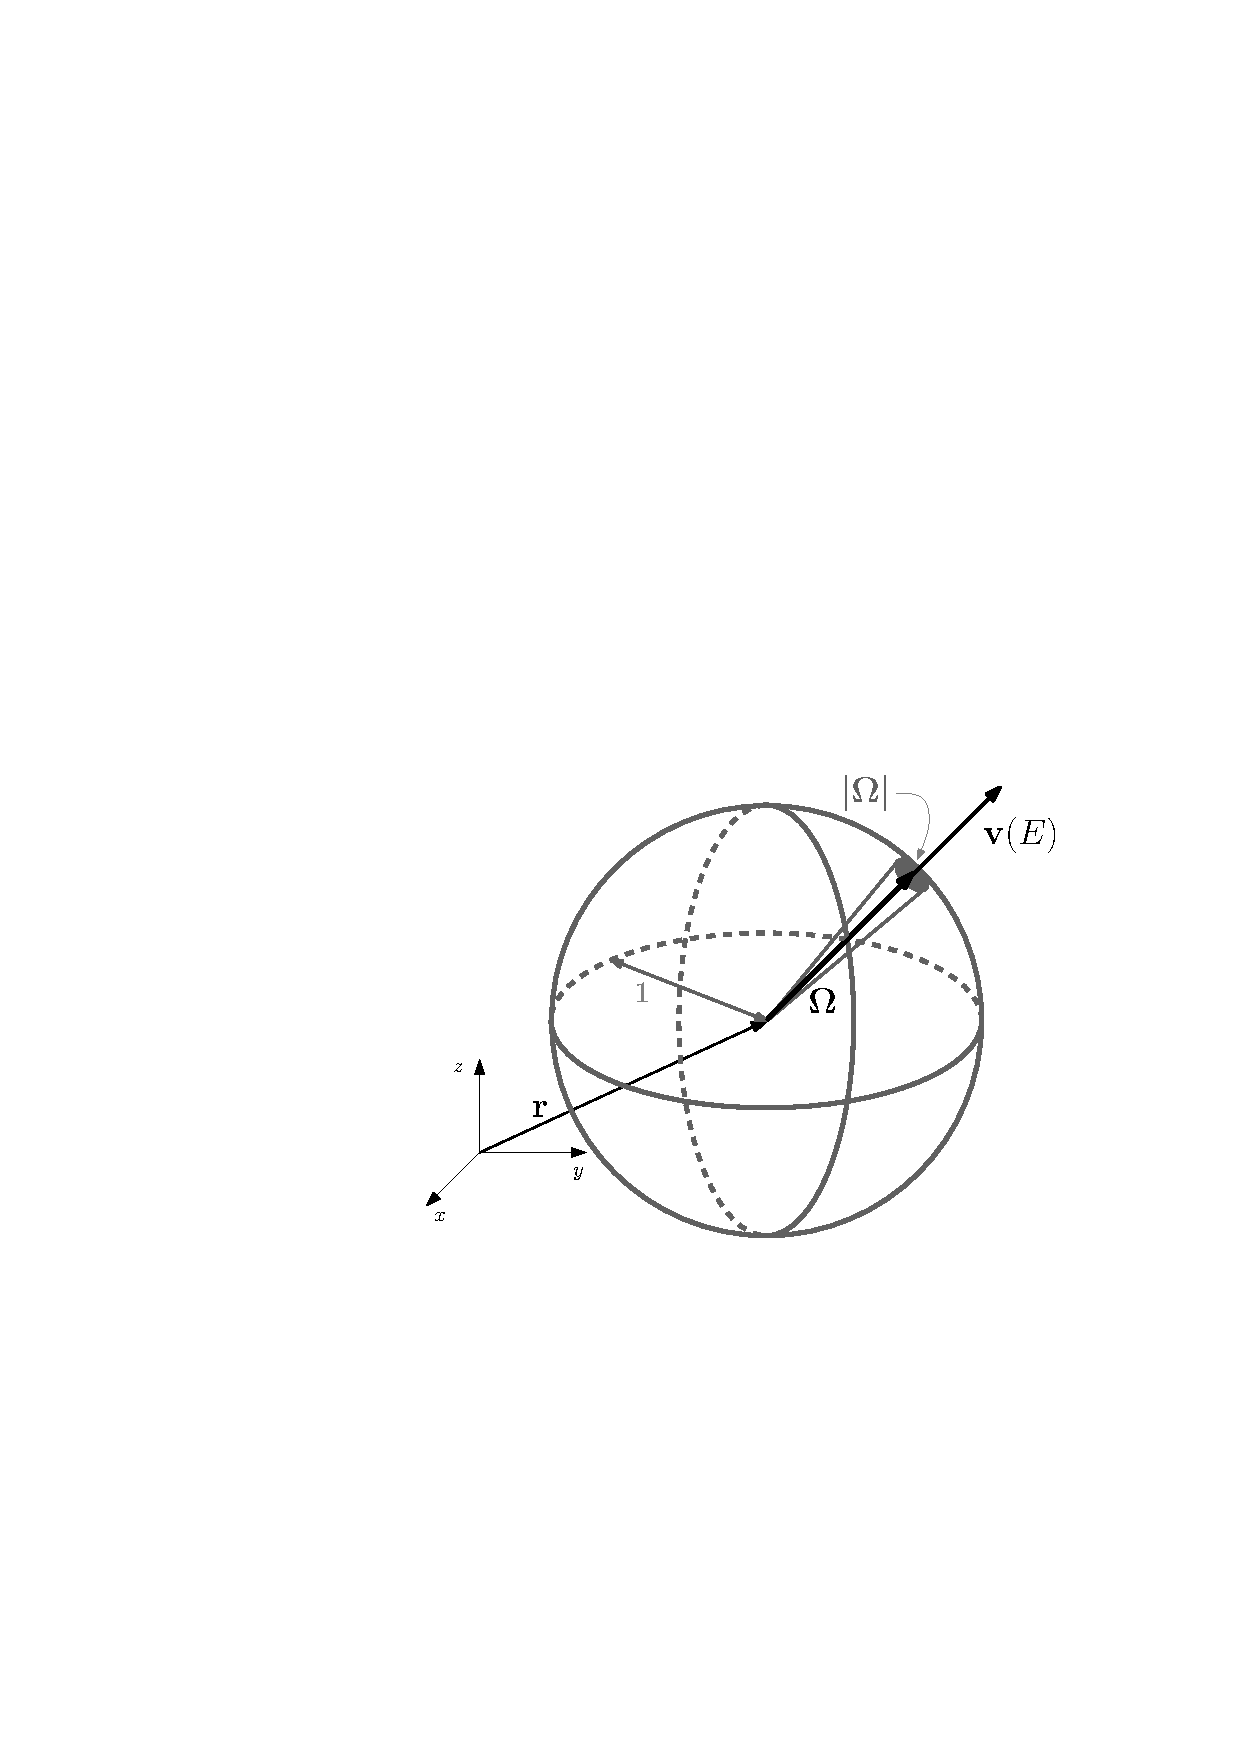
\includegraphics[scale=0.70]{obr/stavovy_prostor}\\[1em]
	\alert{6 dimenzí}
  \end{center}

\end{frame}

\begin{frame}[t]
  \frametitle{Stavový prostor}
  \framesubtitle{Poloha}
 
  $$
    X = \VV \times \EE \times \SS \equiv \{x = (\alert\br,E,\bomega):\ \alert{\br\in \VV}, E \in \EE, \bomega\in \SS\}
  $$
  
  \begin{columns}
  \column{.5\textwidth}
    \centering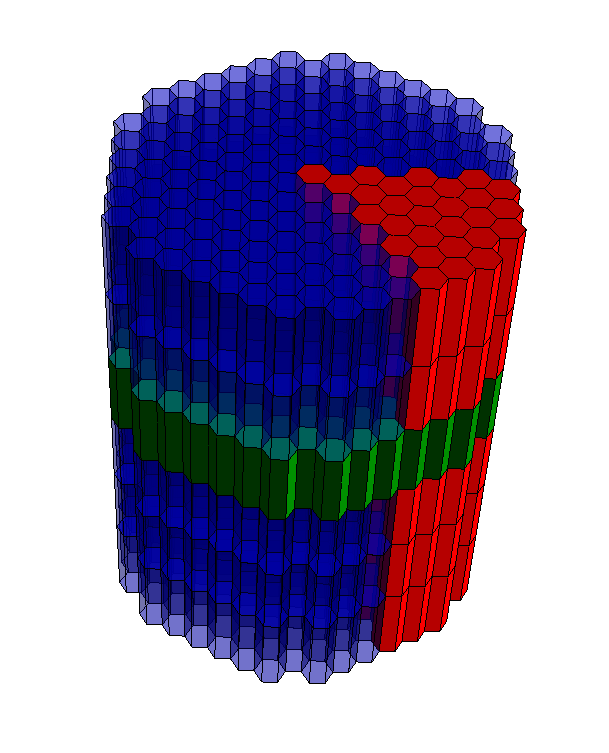
\includegraphics[scale=0.225]{obr/core.png}
  \column{.5\textwidth}
    \includegraphics<1>[scale=0.425]{obr/core/core_level1}
	  \includegraphics<2>[scale=0.425]{obr/core/core_level2}
	  \includegraphics<3>[scale=0.425]{obr/core/core_level3}
	  \includegraphics<4>[scale=0.425]{obr/core/core_level4}
	  \includegraphics<5>[scale=0.425]{obr/core/core_level5}
	  \includegraphics<6>[scale=0.425]{obr/core/core_level6}
	  \includegraphics<7>[scale=0.425]{obr/core/core_level7}
	  \includegraphics<8>[scale=0.425]{obr/core/core_level8}
	  \includegraphics<9>[scale=0.425]{obr/core/core_level9}
	  \includegraphics<10>[scale=0.425]{obr/core/core_level10}
	  \transduration<1-9>{0.5}
	  \transduration<10>{500}    
  \end{columns}
  \hfill\alert{3 dimenze}\hfill\hbox{}
\end{frame}

\begin{frame}[t]
  \frametitle{Stavový prostor}
  \framesubtitle{Energie}
 
  $$
    X = \VV \times \EE \times \SS \equiv \{x = (\br,\alert E,\bomega):\ \br\in \VV, \alert{E \in \EE}, \bomega\in \SS\}
  $$
  \vspace{.5em}
  \begin{columns}
  \column{.5\textwidth}
  \centering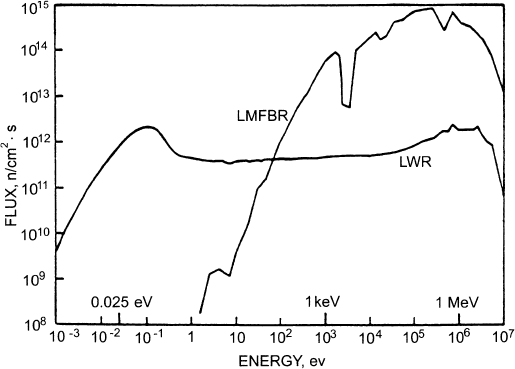
\includegraphics[width=.9\textwidth]{obr/spektrum}
  \column{.5\textwidth}
  \centering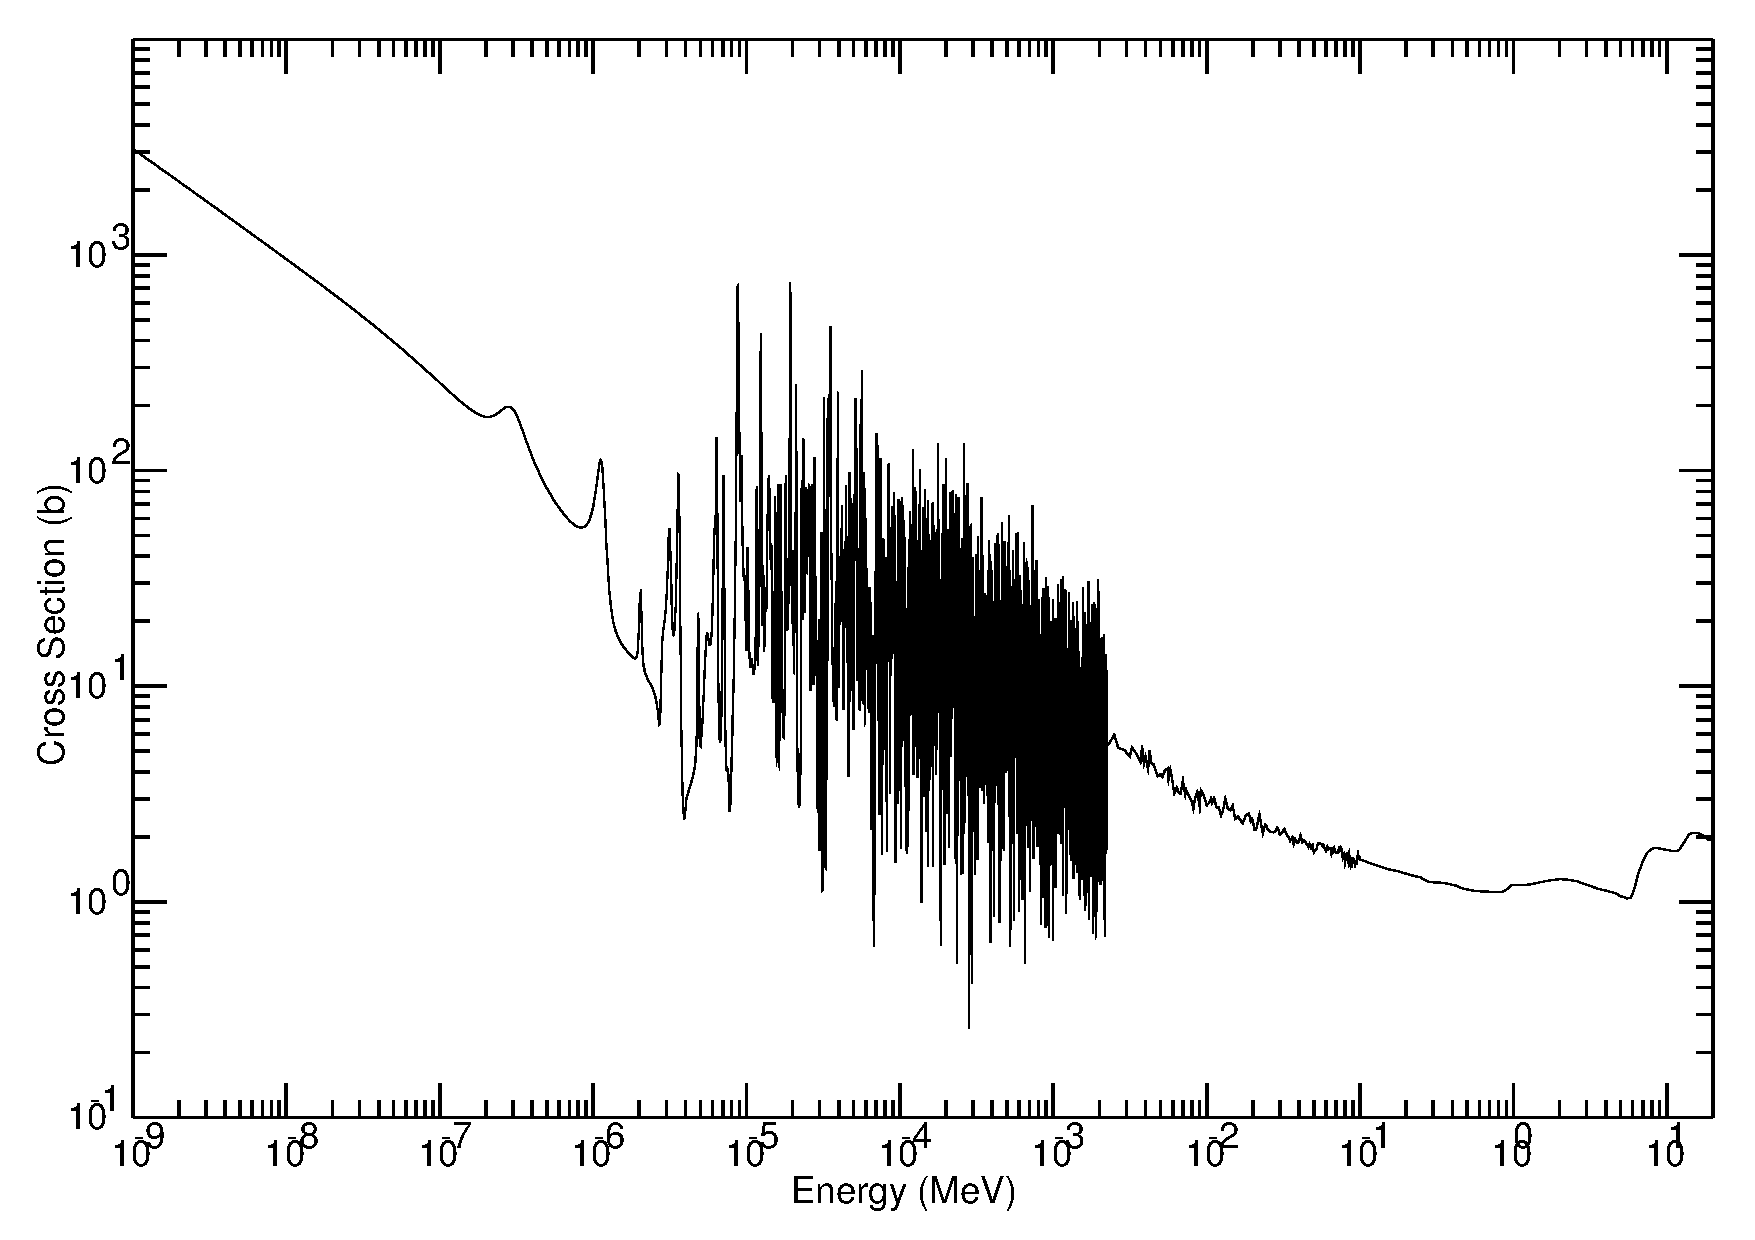
\includegraphics[width=.9\textwidth]{obr/U235f}
  \end{columns}
  \begin{center}
  \alert{1 dimenze}
  \end{center}
\end{frame}

\begin{frame}[t]
  \frametitle{Stavový prostor}
  \framesubtitle{Směr}
 
  $$
    X = \VV \times \EE \times \SS \equiv \{x = (\br,E,\alert\bomega):\ \br\in \VV, E \in \EE, \alert{\bomega\in \SS}\}
  $$
  
  
  \vspace{.5em}
  \begin{columns}
  \column{.5\textwidth}
  \centering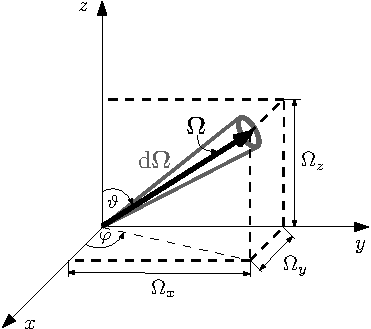
\includegraphics[width=.9\textwidth]{obr/cartesian_streaming}
  \column{.5\textwidth}
  \centering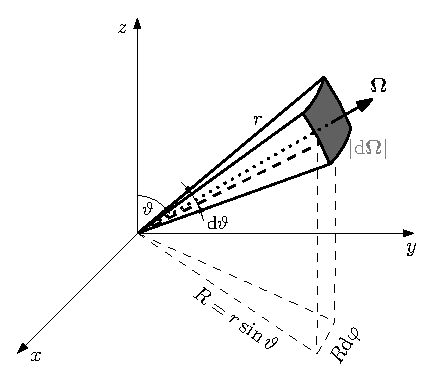
\includegraphics[width=.9\textwidth]{obr/element}
  \end{columns}
  \begin{center}
  \alert{2 dimenze}
  \end{center}
  
\end{frame}

\begin{frame}
  \frametitle{Základní směrově závislé veličiny}

  \begin{columns}[c]
  \begin{column}{.60\linewidth}  
    \begin{itemize}
    \item Hustota neutronů (v $\d{\br}\d{E}\d{\bomega}$):
    \begin{myitemize}
    	\item $N(\br,E,\bomega,t)$
    \end{myitemize}
  \end{itemize}
  \end{column}
  \begin{column}{.30\linewidth}  
  \end{column}
  \end{columns}
  
  \begin{columns}[c]
  \begin{column}{.60\linewidth}
  \begin{itemize}
	  \item Směrový neutronový tok
	  \begin{myitemize}
	    \item $\angflux(\br,E,\bomega,t) = v(E)N(\br,E,\bomega,t)$
	  	\item $\angflux(\br,E,\bomega,t)\,\d{\bomega}\d{E}$
	  \end{myitemize}
  \end{itemize}
  \end{column}
  \begin{column}{.30\linewidth}
  	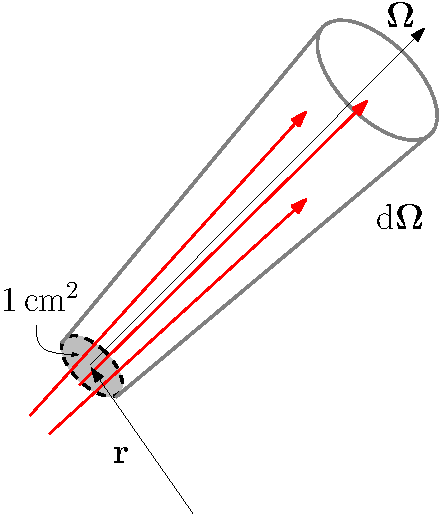
\includegraphics[scale=.45]{obr/angflux}
	\end{column}
	\end{columns}
	\vspace{-2em}
	\begin{columns}
	\begin{column}{.60\linewidth}
	\begin{itemize}
	  \item Směrový neutronový proud
	  \begin{myitemize}
	    \item $\bj(\br,E,\bomega,t) = \bomega \angflux(\br,E,\bomega,t)$\\
	  	\item $j(\br,E,\bomega,t) = \bn\cdot\bj(\br,E,\bomega,t)\,\d{S}\d{\bomega}\d{E}$
	  \end{myitemize}
  \end{itemize}
  \end{column}
  \begin{column}{.30\linewidth}
   	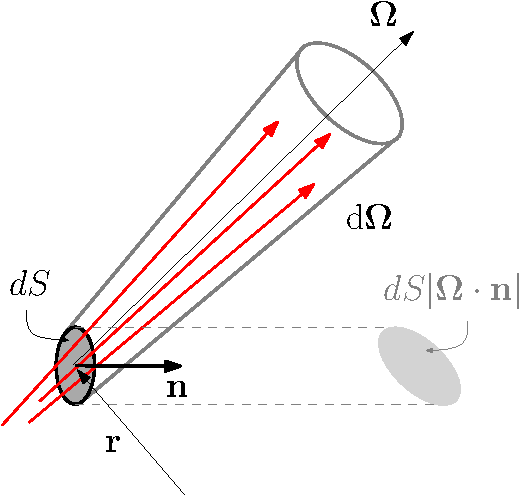
\includegraphics[scale=.45]{obr/angcur}
  \end{column}
  \end{columns}
\end{frame}

\begin{frame}
  \frametitle{Směrově nezávislé veličiny}
  \shorten{-.2em}{-.2em}
  \begin{itemize}
	  \item Skalární neutronový tok:
	    $$ \fl(\br,E,t) = \aint{\angflux(\br,E,\bomega,t)} $$
	  \item Úhrnný neutronový proud: 
	    $$\bJ(\br,E,t)	= \aint{\bj(\br,E,\bomega,t)} = \aint\bomega\angflux(\br,E,\bomega,t)$$
	  \item Parciální neutronový proud:
	    $$
	      j^{\pm}(\br,E,t) = \Aint[\bomega\cdot\bn \gtrless 0]{\abs{\bomega\cdot\bn}\angflux(\br,E,\bomega,t)}
	    $$
	    \vspace*{-.5em}
	  \begin{itemize}
	  	\item přestup neutronů
	  	  $\left.\begin{cases} \mbox{ve směru} &(j^+)\\
	  	    \mbox{proti směru} &(j^-)
	  	    \end{cases}\right\}$
	  	  vnější normály dané plochy
	  \end{itemize}
	  \vspace*{.5em}
	  \item Úhrnný neutronový proud (skalár): $j = \bJ\cdot\bn = j^+-j^-$
  \end{itemize}
\lengthen
\end{frame}

\begin{frame}
  \frametitle{Charakterizace interakcí}
    \begin{myitemize}
	  \item $\Sigma_t = \Sigma_a + \Sigma_f + \Sigma_s$
	  \begin{myitemize}
	  	\item funkce $\br$, $E$, $t$, ale ne $\bomega$ (izotropní prostředí -- stejné vlastnosti ve všech směrech)
	  \end{myitemize}
    \item Četnosti reakcí v objemu $\VV$ za časovou jednotku
	  \begin{myitemize}
	  	\item $\vint{\eint{\Sigma_{t,a,f,s}(\br,E,t)\fl(\br,E,t)}}$
	  \end{myitemize}
	  \item Změna energie a směru pohybu: $\chi(E'\ra E,\, \bomega'\ra\bomega)$
	  \begin{myitemize}
	  	\item štěpení -- \alert<2>{izotropní proces} v \alert<3>{izotropním prostředí}
	  	\begin{itemize}\vspace*{.25em}
	  		\item $\chi(E'\ra E, \alert<3>{\bomega'}\ra\alert<2>{\bomega}) = \alert<2>{\frac{1}{4\pi}}\chi_f(E'\ra E\alert<3>)$
	  	\end{itemize}
	  	\item rozptyl -- \alert<4>{anizotropní proces v izotropním prostředí}
	  	\begin{itemize}\vspace*{.25em}
	  		\item $\chi(E'\ra E, \alert<4>{\bomega'\ra\bomega}) = \chi_s(E'\ra E,\,\alert<4>{\bomega'\cdot\bomega})$
	  	\end{itemize}	  	
	  \end{myitemize}
  \end{myitemize}

\end{frame}


